\documentclass{article}
\iffalse
This file is protected by Copyright. Please refer to the COPYRIGHT file
distributed with this source distribution.

This file is part of OpenCPI <http://www.opencpi.org>

OpenCPI is free software: you can redistribute it and/or modify it under the
terms of the GNU Lesser General Public License as published by the Free Software
Foundation, either version 3 of the License, or (at your option) any later
version.

OpenCPI is distributed in the hope that it will be useful, but WITHOUT ANY
WARRANTY; without even the implied warranty of MERCHANTABILITY or FITNESS FOR A
PARTICULAR PURPOSE. See the GNU Lesser General Public License for more details.

You should have received a copy of the GNU Lesser General Public License along
with this program. If not, see <http://www.gnu.org/licenses/>.
\fi

\author{} % Force author to be blank
%----------------------------------------------------------------------------------------
% Paper size, orientation and margins
%----------------------------------------------------------------------------------------
\usepackage{geometry}
\geometry{
	letterpaper,			% paper type
	portrait,				% text direction
	left=.75in,				% left margin
	top=.75in,				% top margin
	right=.75in,			% right margin
	bottom=.75in			% bottom margin
 }
%----------------------------------------------------------------------------------------
% Header/Footer
%----------------------------------------------------------------------------------------
\usepackage{fancyhdr} \pagestyle{fancy} % required for fancy headers
\renewcommand{\headrulewidth}{0.5pt}
\renewcommand{\footrulewidth}{0.5pt}
\newcommand{\terminaloutput}[1]{\texttt{#1}}
\rhead{\small{Project ANGRYVIPER}}
%----------------------------------------------------------------------------------------
% Appendix packages
%----------------------------------------------------------------------------------------
\usepackage[toc,page]{appendix}
%----------------------------------------------------------------------------------------
% Defined Commands & Renamed Commands
%----------------------------------------------------------------------------------------
\renewcommand{\contentsname}{Table of Contents}
\renewcommand{\listfigurename}{List of Figures}
\renewcommand{\listtablename}{List of Tables}
\newcommand{\todo}[1]{\textcolor{red}{TODO: #1}\PackageWarning{TODO:}{#1}} % To do notes
\newcommand{\code}[1]{\texttt{#1}} % For inline code snippet or command line
%----------------------------------------------------------------------------------------
% Various pacakges
%----------------------------------------------------------------------------------------
\usepackage{hyperref} % for linking urls and lists
\usepackage{graphicx} % for including pictures by file
\usepackage{listings} % for coding language styles
\usepackage{rotating} % for sideways table
\usepackage{pifont}   % for sideways table
\usepackage{pdflscape} % for landscape view
\usepackage{scrextend}
\usepackage{longtable}
\usepackage{setspace}
%----------------------------------------------------------------------------------------
% Table packages
%----------------------------------------------------------------------------------------
\usepackage{tabularx} % c=center,l=left,r=right,X=fill
\usepackage{float}
\floatstyle{plaintop}
\usepackage[tableposition=top]{caption}
\newcolumntype{P}[1]{>{\centering\arraybackslash}p{#1}}
\newcolumntype{M}[1]{>{\centering\arraybackslash}m{#1}}
%----------------------------------------------------------------------------------------
% Block Diagram / FSM Drawings
%----------------------------------------------------------------------------------------
\usepackage{tikz}
\usetikzlibrary{shapes,arrows,fit,positioning}
\usetikzlibrary{automata} % used for the fsm
\usetikzlibrary{calc} % For duplicating clients
\usepgfmodule{oo} % To define a client box
%----------------------------------------------------------------------------------------
% Colors Used
%----------------------------------------------------------------------------------------
\usepackage{colortbl}
\definecolor{blue}{rgb}{.7,.8,.9}
\definecolor{ceruleanblue}{rgb}{0.16, 0.32, 0.75}
\definecolor{drkgreen}{rgb}{0,0.6,0}
\definecolor{deepmagenta}{rgb}{0.8, 0.0, 0.8}
\definecolor{cyan}{rgb}{0.0,0.6,0.6}
\definecolor{maroon}{rgb}{0.5,0,0}
\usepackage{multirow}
%----------------------------------------------------------------------------------------
% Update the docTitle and docVersion per document
%----------------------------------------------------------------------------------------
\def\docTitle{Component Data Sheet}
\def\docVersion{1.3}
%----------------------------------------------------------------------------------------
\date{Version \docVersion} % Force date to be blank and override date with version
\title{\docTitle}
\lhead{\small{\docTitle}}

% find and replace: dev signal, devsignal -> \devsignal{}
\def\devsignal{devsignal}
% find and replace: Dev Signal, Dev signal, dev Signal, DevSignal -> \DevSignal{}
\def\DevSignal{DevSignal}

\def\comp{ad9361\_config\_proxy}
\def\Comp{AD9361 Config Proxy}
\graphicspath{ {figures/} }

\begin{document}

\section*{Summary - \Comp}
\begin{tabular}{|c|M{13.5cm}|}
	\hline
	\rowcolor{blue}
	                  &                  \\
	\hline
	Name              & \comp            \\
	\hline
	Worker Type       & Device Proxy     \\
	\hline
	Version           & v\docVersion{}   \\
	\hline
	Release Date      & Aug 2017         \\
	\hline
	Component Library & ocpi.devices     \\
	\hline
	Workers           & \comp.rcc        \\
	\hline
	Tested Platforms  & Zedboard (Xilinx Linux release xilinx-v14.7\cite{xilinx_linux}), CentOS 7 (via ML605/FMCOMMS3 for FMC LPC slot) \\
	\hline
\end{tabular}
\section*{Functionality}
	The \Comp{} device worker proxy is a software wrapper for Analog Device's No-OS software library\cite{no_os}. No-OS provides command and control of the AD9361 IC\cite{ad9361} via a high-level API which ultimately controls SPI writes to the AD9361 register set. In order to provide functionality analogous to the No-OS API, this worker provides a one-to-one mapping between the No-OS function calls and worker properties.
\section*{Worker Implementation Details}
\subsection*{\comp.rcc}
The version of No-OS used was GitHub commit e9f8fe509cc0e3685cdca47998979f287be4c360\cite{no_os_e9f8fe509cc0e3685cdca47998979f287be4c360}, which was the latest update to the Analog Devices-recommended 2016 R2 release at the time of development. \\ \\
No-OS features "platform layers" which are .c/.h files which implement hardware-specific SPI register accesses within generic API calls. No-OS includes several platform layers which are all specific to the Analog Devices HDL design\cite{adi_hdl_github}. In order to use No-OS with OpenCPI, a new platform layer was added within the \comp{}.rcc code which provided OpenCPI-specific functionality for SPI accesses via slave device property read/writes. This new platform layer was implemented via the ad9361\_platform.cc, ad9361\_platform.h, and parameter.h files. \\
\noindent \begin{sloppypar}
\noindent This worker implements every No-OS API call as a property, with the matching ad9361\_get...()/ad9361\_set...() API calls collapsed into a single volatile and writable \comp{}.rcc property. Each property's type(s)/data structure(s) map directly to the type(s)/data structure(s) passed as argument(s) to that property's analogous No-OS function. The only exception to this methodology are:
\begin{itemize}
	\item The No-OS ad9361\_do\_mcs() function is not implemented as a worker property since it performs a multi-chip-sync operation which could not yet be verified.
	\item The No-OS ad9361\_set\_rx\_fir\_config() / ad9361\_get\_rx\_fir\_config() and ad9361\_set\_tx\_fir\_config() / ad9361\_get\_tx\_fir\_config() functions are implemented as separate \verb+rx_fir_config_write+/\verb+rx_fir_config_read+ and \verb+tx_fir_config_write+/\verb+tx_fir_config_read+ properties, respectively, instead of collapsed into a single rx\_fir\_config and tx\_fir\_config properties due to the fact that the ...get...() calls ignore the ...path\_clks and \_bandwidth struct members, whereas the ..set..() calls do not. Consequently, in an attempt to avoid confusion by the end user, different structs were implemented for the write properties than were for the read properties.
\end{itemize}
\end{sloppypar}
\noindent
The No-OS API calls often require passing integer values which, according to the No-OS documentation, are intended to correlate with C macros. For example, the No-OS ad9361\_set\_rx\_fir\_en\_dis() function has a argument of type uint8\_t, but the comments indicate its value should be one of the ENABLE or DISABLE ad9361\_api.h integer macros:\pagebreak
\begin{lstlisting}
/**
 * Enable/disable the RX FIR filter.
 * @param phy The AD9361 current state structure.
 * @param en_dis The option (ENABLE, DISABLE).
 *               Accepted values:
 *                ENABLE (1)
 *                DISABLE (0)
 * @return 0 in case of success, negative error code otherwise.
 *
 * Note: This function will/may affect the data path.
 */
int32_t ad9361_set_rx_fir_en_dis (struct ad9361_rf_phy *phy,
                                  uint8_t en_dis)
\end{lstlisting}
\begin{sloppypar}
\noindent
Because a design decision was made to have a strict one-to-one mapping between No-OS API calls and \comp{}.rcc properties, and because No-OS passes integers as arguments instead of forcing strictly enumerated types, this worker likewise uses integer types for properties instead of enumerated ones. To aid in alleviating confusion when using this worker's properties, many of the No-OS C macros are mapped to parameter properties of this worker and the property descriptions reference the parameter properties which are intended to be used. This way, parameter properties can be read at runtime, and the read values used to set a property. For example, the \verb+ad9361_set_rx_fir_en_dis+ property's description references the \verb+ENABLE+ and \verb+DISABLE+ parameter properties which have values of 1 and 0, respectively. \\
\end{sloppypar}
In addition to the worker's properties which map to No-OS API calls, other properties exist which provide further functionality. This includes PLL lock status, low-level PLL divider values which can be used to validate the LO frequencies read by No-OS, fastlock memory management (deletion), the FPGA data mode configuration (LVDS, CMOS, etc) via the \verb+LVDS+, \verb+single_port+, \verb+swap_ports+, \verb+half_duplex+, \verb+data_rate_config+ properties, and the \verb+DATA_CLK_P_rate_Hz+.\\ \\
Note also that this worker's usage of no-OS not only makes SPI register accesses but also sets the AD9361 RESETB pin via the ad9361\_config.hdl\cite{config_comp_datasheet} and ad9361\_spi.hdl\cite{spi_comp_datasheet} workers.
\makeatletter
\newcommand{\gettikzxy}[3]{%
  \tikz@scan@one@point\pgfutil@firstofone#1\relax
  \edef#2{\the\pgf@x}%
  \edef#3{\the\pgf@y}%
}
\makeatother
\pgfooclass{clientbox}{ % This is the class clientbox
    \method clientbox() { % The clientbox
    }
    \method apply(#1,#2,#3,#4) { % Causes the clientbox to be shown at coordinate (#1,#2) and named #3
        \node[rectangle,draw=white,fill=white] at (#1,#2) (#3) {#4};
    }
}
\pgfoonew \myclient=new clientbox()
\begin{center}
  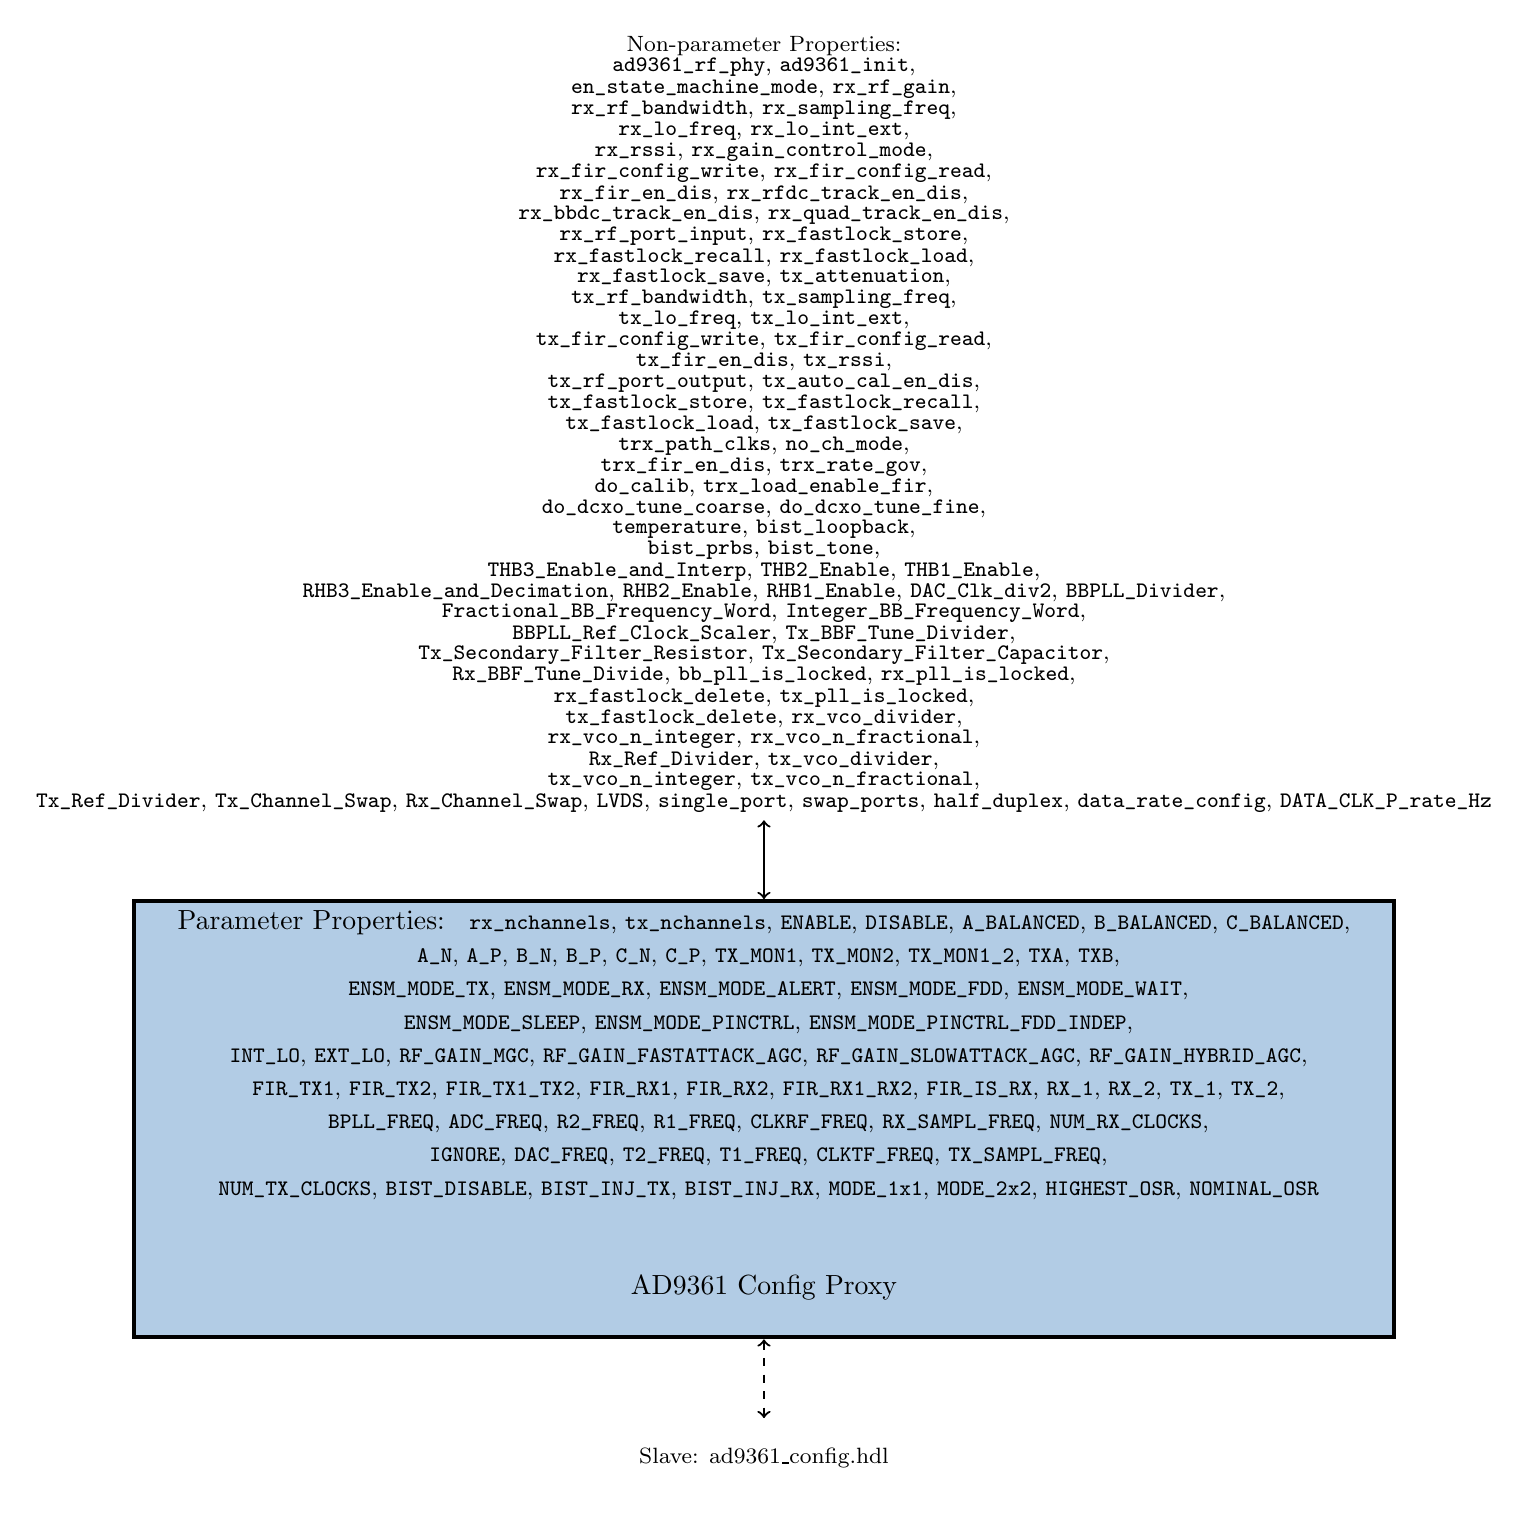
\begin{tikzpicture}[% List of styles applied to all, to override specify on a case-by-case
      every node/.style={
        align=center,      % use this so that the "\\" for line break works
        minimum size=1cm,  % creates space above and below text in rectangle
      },
      every edge/.style={draw,thick}
    ]
    \node[rectangle,ultra thick,draw=black,fill=blue,minimum size=2cm,minimum width=16cm](R1){Parameter Properties: 
\setstretch{0.4}
\fontsize{8}{12}\selectfont
      \verb+rx_nchannels+,
      \verb+tx_nchannels+,
      \verb+ENABLE+,
      \verb+DISABLE+,
      \verb+A_BALANCED+,
      \verb+B_BALANCED+,
      \verb+C_BALANCED+, \\ \setstretch{0.4}
\fontsize{8}{12}\selectfont
      \verb+A_N+,
      \verb+A_P+,
      \verb+B_N+,
      \verb+B_P+,
      \verb+C_N+,
      \verb+C_P+,
      \verb+TX_MON1+,
      \verb+TX_MON2+,
      \verb+TX_MON1_2+,
      \verb+TXA+,
      \verb+TXB+, \\ \setstretch{0.4}
\fontsize{8}{12}\selectfont
      \verb+ENSM_MODE_TX+,
      \verb+ENSM_MODE_RX+,
      \verb+ENSM_MODE_ALERT+,
      \verb+ENSM_MODE_FDD+,
      \verb+ENSM_MODE_WAIT+, \\ \setstretch{0.4}
\fontsize{8}{12}\selectfont
      \verb+ENSM_MODE_SLEEP+,
      \verb+ENSM_MODE_PINCTRL+,
      \verb+ENSM_MODE_PINCTRL_FDD_INDEP+, \\ \setstretch{0.4}
\fontsize{8}{12}\selectfont
      \verb+INT_LO+,
      \verb+EXT_LO+,
      \verb+RF_GAIN_MGC+,
      \verb+RF_GAIN_FASTATTACK_AGC+,
      \verb+RF_GAIN_SLOWATTACK_AGC+,
      \verb+RF_GAIN_HYBRID_AGC+, \\ \setstretch{0.4}
\fontsize{8}{12}\selectfont
      \verb+FIR_TX1+,
      \verb+FIR_TX2+,
      \verb+FIR_TX1_TX2+,
      \verb+FIR_RX1+,
      \verb+FIR_RX2+,
      \verb+FIR_RX1_RX2+,
      \verb+FIR_IS_RX+,
      \verb+RX_1+,
      \verb+RX_2+,
      \verb+TX_1+,
      \verb+TX_2+, \\ \setstretch{0.4}
\fontsize{8}{12}\selectfont
      \verb+BPLL_FREQ+,
      \verb+ADC_FREQ+,
      \verb+R2_FREQ+,
      \verb+R1_FREQ+,
      \verb+CLKRF_FREQ+,
      \verb+RX_SAMPL_FREQ+,
      \verb+NUM_RX_CLOCKS+, \\ \setstretch{0.4}
\fontsize{8}{12}\selectfont
      \verb+IGNORE+,
      \verb+DAC_FREQ+,
      \verb+T2_FREQ+,
      \verb+T1_FREQ+,
      \verb+CLKTF_FREQ+,
      \verb+TX_SAMPL_FREQ+, \\ \setstretch{0.4}
\fontsize{8}{12}\selectfont
      \verb+NUM_TX_CLOCKS+,
      \verb+BIST_DISABLE+,
      \verb+BIST_INJ_TX+,
      \verb+BIST_INJ_RX+,
      \verb+MODE_1x1+,
      \verb+MODE_2x2+,
      \verb+HIGHEST_OSR+,
      \verb+NOMINAL_OSR+
\\ \\ \\ \Comp \\};
    \node[rectangle,draw=white,fill=white](R4)[above= of R1]{ };
\setstretch{0.4}
\fontsize{8}{12}\selectfont
    \node[rectangle,draw=white,fill=white](placeholder)[above= of R1] { Non-parameter Properties:\\ 
   			\verb+ad9361_rf_phy+,
			\verb+ad9361_init+, \\
			\verb+en_state_machine_mode+,
			\verb+rx_rf_gain+, \\
			\verb+rx_rf_bandwidth+,
			\verb+rx_sampling_freq+, \\
			\verb+rx_lo_freq+,
			\verb+rx_lo_int_ext+, \\
			\verb+rx_rssi+,
			\verb+rx_gain_control_mode+, \\
			\verb+rx_fir_config_write+,
			\verb+rx_fir_config_read+, \\
			\verb+rx_fir_en_dis+,
			\verb+rx_rfdc_track_en_dis+, \\
			\verb+rx_bbdc_track_en_dis+,
			\verb+rx_quad_track_en_dis+, \\
			\verb+rx_rf_port_input+,
			\verb+rx_fastlock_store+, \\
			\verb+rx_fastlock_recall+,
			\verb+rx_fastlock_load+, \\
			\verb+rx_fastlock_save+,
			\verb+tx_attenuation+, \\
			\verb+tx_rf_bandwidth+,
			\verb+tx_sampling_freq+, \\
			\verb+tx_lo_freq+,
			\verb+tx_lo_int_ext+, \\
			\verb+tx_fir_config_write+,
			\verb+tx_fir_config_read+, \\
			\verb+tx_fir_en_dis+,
			\verb+tx_rssi+, \\
			\verb+tx_rf_port_output+,
			\verb+tx_auto_cal_en_dis+, \\
			\verb+tx_fastlock_store+,
			\verb+tx_fastlock_recall+, \\
			\verb+tx_fastlock_load+,
			\verb+tx_fastlock_save+, \\
			\verb+trx_path_clks+,
			\verb+no_ch_mode+, \\
			\verb+trx_fir_en_dis+,
			\verb+trx_rate_gov+, \\
			\verb+do_calib+,
			\verb+trx_load_enable_fir+, \\
			\verb+do_dcxo_tune_coarse+,
			\verb+do_dcxo_tune_fine+, \\
			\verb+temperature+,
			\verb+bist_loopback+, \\
			\verb+bist_prbs+,
			\verb+bist_tone+, \\
			\verb+THB3_Enable_and_Interp+,
			\verb+THB2_Enable+,
			\verb+THB1_Enable+, \\
			\verb+RHB3_Enable_and_Decimation+,
			\verb+RHB2_Enable+,
			\verb+RHB1_Enable+,
			\verb+DAC_Clk_div2+,
			\verb+BBPLL_Divider+, \\
			\verb+Fractional_BB_Frequency_Word+,
			\verb+Integer_BB_Frequency_Word+, \\
			\verb+BBPLL_Ref_Clock_Scaler+,
			\verb+Tx_BBF_Tune_Divider+, \\
			\verb+Tx_Secondary_Filter_Resistor+,
			\verb+Tx_Secondary_Filter_Capacitor+, \\
			\verb+Rx_BBF_Tune_Divide+,
			\verb+bb_pll_is_locked+,
			\verb+rx_pll_is_locked+, \\
			\verb+rx_fastlock_delete+,
			\verb+tx_pll_is_locked+, \\
			\verb+tx_fastlock_delete+,
			\verb+rx_vco_divider+, \\
			\verb+rx_vco_n_integer+,
			\verb+rx_vco_n_fractional+, \\
			\verb+Rx_Ref_Divider+,
			\verb+tx_vco_divider+, \\
			\verb+tx_vco_n_integer+,
			\verb+tx_vco_n_fractional+, \\
			\verb+Tx_Ref_Divider+,
			\verb+Tx_Channel_Swap+,
			\verb+Rx_Channel_Swap+,
			\verb+LVDS+,
			\verb+single_port+,
			\verb+swap_ports+,
			\verb+half_duplex+,
			\verb+data_rate_config+,
			\verb+DATA_CLK_P_rate_Hz+
};
    \node[rectangle,draw=white,fill=white](R2)[below= of R1] { Slave: ad9361\_config.hdl};
    \path[<->]
  (R1)edge [] node [] {} (R4);
    \path[<->,dashed]
  (R1)edge [] node [] {} (R2)
    ;
  \end{tikzpicture}
\end{center}
\section*{Source Dependencies}
\subsection*{\comp.rcc}
\begin{itemize}
	\item opencpi/hdl/devices/\comp{}.rcc/\comp{}.cc
	\item opencpi/hdl/devices/\comp{}.rcc/ad9361\_platform.cc
	\item opencpi/hdl/devices/\comp{}.rcc/ad9361\_platform.h
	\item opencpi/hdl/devices/\comp{}.rcc/parameters.h
	\item libad9361.a (no-OS static library installed with OpenCPI prerequisites)
\end{itemize}
\begin{landscape}

	\section*{Component Spec Properties}
	\begin{scriptsize}
		\begin{longtable}{|p{3.6cm}|p{8.1cm}|p{1.4cm}|p{1.3cm}|p{1.4cm}|p{2.5cm}|p{3.6cm}|}
			\hline
			\rowcolor{blue}
			Name               & Type & Array Dimensions & Accessibility      & Valid Range & Default & Usage                                                                               \\
			\hline
      \verb+rx_nchannels+              & UChar        & -               & Parameter             & Standard                         & 2                   & - \\
			\hline
      \verb+tx_nchannels+              & UChar        & -               & Parameter             & Standard                         & 2                   & - \\
			\hline
      \verb+ENABLE+                    & UChar        & -               & Parameter             & Standard                         & 1                   & - \\
			\hline
      \verb+DISABLE+                   & UChar        & -               & Parameter             & Standard                         & 0                   & - \\
			\hline
      \verb+A_BALANCED+                & ULong        & -               & Parameter             & Standard                         & 0                   & - \\
			\hline
      \verb+B_BALANCED+                & ULong        & -               & Parameter             & Standard                         & 1                   & - \\
			\hline
      \verb+C_BALANCED+                & ULong        & -               & Parameter             & Standard                         & 2                   & - \\
			\hline
      \verb+A_N+                       & ULong        & -               & Parameter             & Standard                         & 3                   & - \\
			\hline
      \verb+A_P+                       & ULong        & -               & Parameter             & Standard                         & 4                   & - \\
			\hline
      \verb+B_N+                       & ULong        & -               & Parameter             & Standard                         & 5                   & - \\
			\hline
      \verb+B_P+                       & ULong        & -               & Parameter             & Standard                         & 6                   & - \\
			\hline
      \verb+C_N+                       & ULong        & -               & Parameter             & Standard                         & 7                   & - \\
			\hline
      \verb+C_P+                       & ULong        & -               & Parameter             & Standard                         & 8                   & - \\
			\hline
      \verb+TX_MON1+                   & ULong        & -               & Parameter             & Standard                         & 9                   & - \\
			\hline
      \verb+TX_MON2+                   & ULong        & -               & Parameter             & Standard                         & 10                  & - \\
			\hline
      \verb+TX_MON1_2+                 & ULong        & -               & Parameter             & Standard                         & 11                  & - \\
			\hline
      \verb+TXA+                       & ULong        & -               & Parameter             & Standard                         & 0                   & - \\
			\hline
      \verb+TXB+                       & ULong        & -               & Parameter             & Standard                         & 1                   & - \\
			\hline
      \verb+ENSM_MODE_TX+              & Long         & -               & Parameter             & Standard                         & 0                   & - \\
			\hline
      \verb+ENSM_MODE_RX+              & Long         & -               & Parameter             & Standard                         & 1                   & - \\
			\hline
      \verb+ENSM_MODE_ALERT+           & Long         & -               & Parameter             & Standard                         & 2                   & - \\
			\hline
      \verb+ENSM_MODE_FDD+             & Long         & -               & Parameter             & Standard                         & 3                   & - \\
			\hline
      \verb+ENSM_MODE_WAIT+            & Long         & -               & Parameter             & Standard                         & 4                   & - \\
			\hline
      \verb+ENSM_MODE_SLEEP+           & Long         & -               & Parameter             & Standard                         & 5                   & - \\
			\hline
      \verb+ENSM_MODE_PINCTRL+         & Long         & -               & Parameter             & Standard                         & 6                   & - \\
			\hline
      \verb+ENSM_MODE_PINCTRL_FDD_INDEP+&Long         & -               & Parameter             & Standard                         & 7                   & - \\
			\hline
      \verb+INT_LO+                    & UChar        & -               & Parameter             & Standard                         & 0                   & - \\
			\hline
      \verb+EXT_LO+                    & UChar        & -               & Parameter             & Standard                         & 1                   & - \\
			\hline
      \verb+RF_GAIN_MGC+               & UChar        & -               & Parameter             & Standard                         & 0                   & - \\
			\hline
      \verb+RF_GAIN_FASTATTACK_AGC+    & UChar        & -               & Parameter             & Standard                         & 1                   & - \\
			\hline
      \verb+RF_GAIN_SLOWATTACK_AGC+    & UChar        & -               & Parameter             & Standard                         & 2                   & - \\
			\hline
      \verb+RF_GAIN_HYBRID_AGC+        & UChar        & -               & Parameter             & Standard                         & 3                   & - \\
			\hline
      \verb+FIR_TX1+                   & UChar        & -               & Parameter             & Standard                         & 0x01                & - \\
			\hline
      \verb+FIR_TX2+                   & UChar        & -               & Parameter             & Standard                         & 0x02                & - \\
			\hline
      \verb+FIR_TX1_TX2+               & UChar        & -               & Parameter             & Standard                         & 0x03                & - \\
			\hline
      \verb+FIR_RX1+                   & UChar        & -               & Parameter             & Standard                         & 0x81                & - \\
			\hline
      \verb+FIR_RX2+                   & UChar        & -               & Parameter             & Standard                         & 0x82                & - \\
			\hline
      \verb+FIR_RX1_RX2+               & UChar        & -               & Parameter             & Standard                         & 0x83                & - \\
			\hline
      \verb+FIR_IS_RX+                 & UChar        & -               & Parameter             & Standard                         & 0x80                & - \\
			\hline
      \verb+RX_1+                      & UChar        & -               & Parameter             & Standard                         & 1                   & - \\
			\hline
      \verb+RX_2+                      & UChar        & -               & Parameter             & Standard                         & 2                   & - \\
			\hline
      \verb+TX_1+                      & UChar        & -               & Parameter             & Standard                         & 1                   & - \\
			\hline
      \verb+TX_2+                      & UChar        & -               & Parameter             & Standard                         & 2                   & - \\
			\hline
      \verb+BPLL_FREQ+                 & UChar        & -               & Parameter             & Standard                         & 0                   & - \\
			\hline
      \verb+ADC_FREQ+                  & UChar        & -               & Parameter             & Standard                         & 1                   & - \\
			\hline
      \verb+R2_FREQ+                   & UChar        & -               & Parameter             & Standard                         & 2                   & - \\
			\hline
      \verb+R1_FREQ+                   & UChar        & -               & Parameter             & Standard                         & 3                   & - \\
			\hline
      \verb+CLKRF_FREQ+                & UChar        & -               & Parameter             & Standard                         & 4                   & - \\
			\hline
      \verb+RX_SAMPL_FREQ+             & UChar        & -               & Parameter             & Standard                         & 5                   & - \\
			\hline
      \verb+NUM_RX_CLOCKS+             & UChar        & -               & Parameter             & Standard                         & 6                   & - \\
			\hline
      \verb+IGNORE+                    & UChar        & -               & Parameter             & Standard                         & 0                   & - \\
			\hline
      \verb+DAC_FREQ+                  & UChar        & -               & Parameter             & Standard                         & 1                   & - \\
			\hline
      \verb+T2_FREQ+                   & UChar        & -               & Parameter             & Standard                         & 2                   & - \\
			\hline
      \verb+T1_FREQ+                   & UChar        & -               & Parameter             & Standard                         & 3                   & - \\
			\hline
      \verb+CLKTF_FREQ+                & UChar        & -               & Parameter             & Standard                         & 4                   & - \\
			\hline
      \verb+TX_SAMPL_FREQ+             & UChar        & -               & Parameter             & Standard                         & 5                   & - \\
			\hline
      \verb+NUM_TX_CLOCKS+             & UChar        & -               & Parameter             & Standard                         & 6                   & - \\
			\hline
      \verb+BIST_DISABLE+              & ULong        & -               & Parameter             & Standard                         & 0                   & - \\
			\hline
      \verb+BIST_INJ_TX+               & ULong        & -               & Parameter             & Standard                         & 1                   & - \\
			\hline
      \verb+BIST_INJ_RX+               & ULong        & -               & Parameter             & Standard                         & 2                   & - \\
			\hline
      \verb+MODE_1x1+                  & UChar        & -               & Parameter             & Standard                         & 1                   & - \\
			\hline
      \verb+MODE_2x2+                  & UChar        & -               & Parameter             & Standard                         & 2                   & - \\
			\hline
      \verb+HIGHEST_OSR+               & ULong        & -               & Parameter             & Standard                         & 0                   & - \\
			\hline
      \verb+NOMINAL_OSR+               & ULong        & -               & Parameter             & Standard                         & 2                   & - \\
			\hline
			\verb+ad9361_rf_phy+ & Struct (see \hyperlink{tab1}{Table 1})  & - & Volatile & Standard & - & - \\
			\hline
			\verb+ad9361_init+ & Struct (see \hyperlink{tab2}{Table 2}) & - & Initial & Standard & \begin{tabular}{l}reference\_clk\_rate 4\\0e6,one\_rx\_one\_tx\_m\\ode\_use\_rx\_num 1,o\\ne\_rx\_one\_tx\_mode\_\\use\_tx\_num 1,frequ\\ency\_division\_duple\\x\_mode\_enable 1,xo\\\_disable\_use\_ext\_ref\\clk\_enable 0,two\_t\_\\two\_r\_timing\_enable\\ 0,pp\_tx\_swap\_enable\\ 1,pp\_rx\_swap\_enable\\ 1,tx\_channel\_swap\_e\\nable 1,rx\_channel\_s\\wap\_enable 1,delay\_\\rx\_data 0,rx\_data\_cl\\ock\_delay 0,rx\_data\_\\delay 4,tx\_fb\_clock\_\\delay 7,tx\_data\_dela\\y 0\end{tabular} & Initialize the AD9361 part. \\
			\hline   
			\verb+en_state_machine_mode+ & ULong & - & Volatile, Writable & Standard & \verb+ENSM_MODE_ALERT+ & Get/set the Enable State Machine (ENSM) mode. Value should be set using one of the ENSM\_MODE\_ parameters.\\
			\hline
			\verb+rx_rf_gain+ & Long & \verb+rx_nchannels+ & Volatile, Writable & Standard & 0,0 & Get/set the receive RF gain for the selected channel. The gain is in dB. Note that the written value to the second index of this property will not be applied when this worker's ad9361\_rf\_phy.pdata.rx2tx2 property member is false.\\
			\hline
			\verb+rx_rf_bandwidth+ & ULong & - & Volatile, Writable & Standard & 18e6 & Get/set the RX RF bandwidth. The bandwidth is in Hz.\\
			\hline
			\verb+rx_sampling_freq+ & ULong & - & Volatile, Writable & Standard & 30.72e6 & Get the RX sampling frequency. The frequency is in Hz. \\
			\hline
			\verb+rx_lo_freq+ & ULongLong & - & Volatile, Writable & Standard & 2.4e9 & Get/set the RX LO frequency. The frequency is in Hz. \\
			\hline
			\verb+rx_lo_int_ext+ & Char & - & Readble, Writable & Standard & \verb+INT_LO+ & Switch between the internal and external LO. The RX LO is affected. \\
			\hline
			\verb+rx_rssi+ & Struct (see \hyperlink{tab3}{Table 3}) & \verb+rx_nchannels+ & Volatile & Standard & - & Get the RSSI for the selected channel. \\
			\hline
			\verb+rx_gain_control_mode+ & UChar & \verb+rx_nchannels+ & Volatile, Writable & Standard & \verb+RF_GAIN_MGC+, \verb+RF_GAIN_MGC+ & Get/set the gain control mode for the selected channel. Note that, when this worker's ad9361\_rf\_phy.pdata.rx2tx2 property member is false, the value read from the second index of this property should be ignored and the value written to the second index won't be applied. \\
			\hline
			\verb+rx_fir_config_write+ & \begin{tabular}{|p{2.2cm}|p{2.7cm}|p{2cm}|} \hline \cellcolor{blue} Name & \cellcolor{blue}Type & \cellcolor{blue} ArrayLength \\ \hline rx & ULong & - \\ \hline rx\_gain & Long & - \\ \hline rx\_dec & ULong & - \\ \hline rx\_coef & Short & 128 \\ \hline rx\_coef\_size & UChar & - \\ \hline\end{tabular} & - & Writable & Standard & \begin{tabular}{l}rx 0x83,rx\_gain 0,rx\\\_dec 1,rx\_coef \{1,0,0\\,0,0,0,0,0,0,0,0,0,0,0\\,0,0,0,0,0,0,0,0,0,0,0\\,0,0,0,0,0,0,0,0,0,0,0\\,0,0,0,0,0,0,0,0,0,0,0\\,0,0,0,0,0,0,0,0,0,0,0\\,0,0,0,0,0,0,0,0,0,0,0\\,0,0,0,0,0,0,0,0,0,0,0\\,0,0,0,0,0,0,0,0,0,0,0\\,0,0,0,0,0,0,0,0,0,0,0\\,0,0,0,0,0,0,0,0,0,0,0\\,0,0,0,0,0,0,0,0,0,0,0\\,0,0,0,0\},rx\_coef\_siz\\e 128\end{tabular} & - \\
			\hline
			\verb+rx_fir_config_read+ & \begin{tabular}{|p{2.2cm}|p{2.7cm}|p{2cm}|} \hline \cellcolor{blue} Name & \cellcolor{blue}Type & \cellcolor{blue} ArrayLength \\ \hline rx\_gain & Long & - \\ \hline rx\_dec & ULong & - \\ \hline rx\_coef & Short & 128 \\ \hline rx\_coef\_size & UChar & - \\ \hline \end{tabular} & \verb+rx_nchannels+ & Volatile & Standard & - & Note that the readback value of the second index of this property should be ignored when this worker's ad9361\_rf\_phy.pdata.rx2tx2 property member is false. \\
			\hline
			\verb+rx_fir_en_dis+ & UChar & - & Volatile, Writable & Standard & \verb+DISABLE+ & Get/set the status of the RX FIR filter. The status is one of the parameter values ENABLE or DISABLE. \\
			\hline
			\verb+rx_rfdc_track_en_dis+ & UChar & - & Volatile, Writable & Standard & \verb+DISABLE+ & Get/set the status of the RX RFDC Tracking. The status is one of the parameter values ENABLE or DISABLE.\\
			\hline
			\verb+rx_bbdc_track_en_dis+ & UChar & - & Volatile, Writable & Standard & \verb+DISABLE+ & Get/set the status of the RX BasebandDC Tracking. The status is one of the parameter values ENABLE or DISABLE.\\
			\hline
			\verb+rx_quad_track_en_dis+ & UChar & - & Volatile, Writable & Standard & \verb+DISABLE+ & Get/set the status of the RX Quadrate Tracking. The status is one of the parameter values ENABLE or DISABLE. \\
			\hline
			\verb+rx_rf_port_input+ & ULong & - & Volatile, Writable & Standard & \verb+A_BALANCED+ & Get/set the RX RF input port. \\
			\hline
			\verb+rx_fastlock_store+ & ULong & - & Writable & Standard & - & Store RX fastlock profile. Writing a value will initiate the process of creating an RX fast lock profile and store it in the AD9361 in the RX profile index indicated by the value written. \\
			\hline
			\verb+rx_fastlock_recall+ & ULong & - & Writable & Standard & - & Recall specified RX fastlock profile. Writing a value will initiate the process of applying an RX fast lock profile that was previously stored inside the AD9361. The written value indicates the index of the RX profile to be applied. \\
			\hline
			\verb+rx_fastlock_load+ & Struct (see \hyperlink{tab4}{Table 4}) & - & Writable & Standard & - & - \\
			\hline
			\verb+rx_fastlock_save+ & Struct (see \hyperlink{tab5}{Table 5}) & - & Writable & Standard & - & - \\
			\hline
			\verb+tx_attenuation+ & ULong & \verb+tx_nchannels+ & Volatile, Writable & Standard & 1000, 1000 & Get/set the transmit attenuation for the selected channel. The attenuation is in millidB. Values written will be rounded down to the nearest 250 millidB. Note that the written value to the second index of this property will not be applied when this worker's ad9361\_rf\_phy.pdata.rx2tx2 property member is false. \\
			\hline
			\verb+tx_rf_bandwidth+ & ULong & - & Volatile, Writable & Standrad & 18e6 & Get/set the TX RF bandwidth. The bandwidth is in Hz. \\
			\hline
			\verb+tx_sampling_freq+ & ULong & - & Volatile, Writable & Standard & 30.72e6 & Get/set the TX sampling frequency. The frequency is in Hz. \\
			\hline
			\verb+tx_lo_freq+ & ULongLong & - & Volatile, Writable & Standard & 2.4e9 & Get/set the TX LO frequency. The frequency is in Hz. \\
			\hline
			\verb+tx_lo_int_ext+ & UChar & - & Readable, Writable & Standard & \verb+INT_LO+ & Switch between the internal and external LO. The TX LO is affected. \\
			\hline
			\verb+tx_fir_config_write+ & \begin{tabular}{|p{2.2cm}|p{2.7cm}|p{1.7cm}|} \hline \cellcolor{blue} Name & \cellcolor{blue}Type & \cellcolor{blue} ArrayLength \\ \hline tx & ULong & - \\ \hline tx\_gain & Long & - \\ \hline tx\_int & ULong & - \\ \hline tx\_coef & Short & 128 \\ \hline tx\_coef\_size & UChar & - \\ \hline\end{tabular} & - & Writable & Standard & \begin{tabular}{l}tx 0x03,tx\_gain 0,tx\\\_int 1,tx\_coef \{1,0,0\\,0,0,0,0,0,0,0,0,0,0,0\\,0,0,0,0,0,0,0,0,0,0,0\\,0,0,0,0,0,0,0,0,0,0,0\\,0,0,0,0,0,0,0,0,0,0,0\\,0,0,0,0,0,0,0,0,0,0,0\\,0,0,0,0,0,0,0,0,0,0,0\\,0,0,0,0,0,0,0,0,0,0,0\\,0,0,0,0,0,0,0,0,0,0,0\\,0,0,0,0,0,0,0,0,0,0,0\\,0,0,0,0,0,0,0,0,0,0,0\\,0,0,0,0,0,0,0,0,0,0,0\\,0,0,0,0\},rx\_coef\_siz\\e 128\end{tabular} & - \\
			\hline
			\verb+tx_fir_config_read+ & \begin{tabular}{|p{2.2cm}|p{2.7cm}|p{1.7cm}|} \hline \cellcolor{blue} Name & \cellcolor{blue}Type & \cellcolor{blue}ArrayLength \\ \hline tx\_gain & Long & -\\ \hline tx\_int & ULong & -\\ \hline tx\_coef & Short & 128 \\ \hline tx\_coef\_size & UChar & - \\ \hline \end{tabular} & \verb+tx_nchannels+ & Volatile & Standard & - & Note that the readback value of the second index of this property should be ignored when this worker's ad9361\_rf\_phy.pdata.rx2tx2 property member is false. \\
			\hline
			\verb+tx_fir_en_dis+ & UChar & - & Volatile, Writable & Stabdard & \verb+DISABLE+ & Get/set the status of the TX FIR filter. The status is one of the parameter values ENABLE or DISABLE. \\
			\hline
			\verb+tx_rssi+ & ULong & \verb+tx_nchannels+ & Volatile & Standard & - & Get the TX RSSI for the selected channel. The value read represents the RSSI in millidB. Note that the readback value of the second index of this property should be ignored when this worker's ad9361\_rf\_phy.pdata.rx2tx2 property member is false. \\
			\hline
			\verb+tx_rf_port_output+ & ULong & - & Volatile, Writable & Standard & \verb+TXA+ & Get/set the TX RF output port. \\
			\hline
			\verb+tx_auto_cal_en_dis+ & UChar & - & Volatile, Writable & Standard & \verb+DISABLE+ & Get/set the status of the auto calibration flag. The value should be one of the parameter values ENABLE or DISABLE. \\
			\hline
			\verb+tx_fastlock_store+ & ULong & - & Writable & Standard & - & Store TX fastlock profile. Writing a value will initiate the process of creating a TX fast lock profile and store it in the AD9361 in the TX profile index indicated by the value written. \\
			\hline
			\verb+tx_fastlock_recall+ &  ULong & - & Writable & Standard & - & Recall specified TX fastlock profile. Writing a value will initiate the process of applying an TX fast lock profile that was previously stored inside the AD9361. The written value indicates the index of the TX profile to be applied. \\
			\hline
			\verb+tx_fastlock_load+ & Struct (see \hyperlink{tab6}{Table 6}) & - & Writable & Standard & - & - \\
			\hline
			\verb+tx_fastlock_save+ & Struct (see \hyperlink{tab7}{Table 7}) & - & Writable & Standard & - & - \\
			\hline
			\verb+trx_path_clks+ & Struct (see \hyperlink{tab8}{Table 8}) & - & Volatile, Writable & Standard & - & Set the RX and TX path rates. \\
			\hline
			\verb+no_ch_mode+ & UChar & - & Writable & Standard & - & Set the number of channels mode. Accepted values are one of the parameter values MODE\_1x1 or MODE\_2x2. \\
			\hline
			\verb+trx_fir_en_dis+ & UChar & - & Writable & Standard & - & Enable/disable the TRX FIR filters. Accepted values are one of the parameter values ENABLE or DISABLE.\\
			\hline
			\verb+trx_rate_gov+ & ULong & - & Volatile, Writable & Standard & - & Get/set the OSR rate governor. Accepted values are one of the parameter values HIGHEST\_OSR or NOMINAL\_OSR. \\
			\hline
			\verb+do_calib+ & Struct (see \hyperlink{tab9}{Table 9})  & - & Writable & Standard & - & Perform the selected calibration. \\
			\hline
			\verb+trx_load_enable_fir+ & \begin{tabular}{|p{2.2cm}|p{2.7cm}|p{1.7cm}|} \hline \cellcolor{blue} Name & \cellcolor{blue}Type & \cellcolor{blue} ArrayLength \\ \hline rx & ULong & - \\ \hline rx\_gain & Long & - \\ \hline rx\_dec & ULong & - \\ \hline rx\_coef & Short & - \\ \hline rx\_coef\_size & UChar & 128 \\ \hline rx\_path\_clks & UChar & 6 \\ \hline rx\_bandwidth & UChar & - \\ \hline tx & ULong & - \\ \hline tx\_gain & Long & - \\ \hline tx\_int & ULong & - \\ \hline tx\_coef & Short & 128 \\ \hline tx\_coef\_size & UChar & - \\ \hline tx\_path\_clks & UChar & 6 \\ \hline tx\_bandwidth & UChar & - \\ \hline\end{tabular} & - & Writable & Standard & - & Load and enable TRX FIR filters configurations. \\
			\hline
			\verb+do_dcxo_tune_coarse+ & ULong & - & Writable & Standard & - & Do DCXO coarse tuning.\\
			\hline
			\verb+do_dcxo_tune_fine+ & ULong & - & Writable & Standard & - & Do DCXO fine tuning. \\
			\hline
			\verb+temperature+ & Long & - & Volatile & Standard & - & Get the temperature. \\
			\hline
			\verb+bist_loopback+ & Long & - & Volatile, Writable & Standard & - & BIST loopback mode. Valid values are 0 (disables loopback), 1 (loopback AD9361 internal TX-RX), or 2 (loopback (FPGA internal RX-.TX). While a value of 2 is handled by no-os, it is not expected to work with OpenCPI's AD9361 device workers \\
			\hline
			\verb+bist_prbs+ & UChar & - & Volatile, Writable & Standard & - & BIST mode. Valid values are either BIST\_DISABLE or BIST\_INJ\_RX. \\
			\hline
			\verb+bist_tone+ & Struct (see \hyperlink{tab10}{Table 10}) & - & Volatile, Writable & Standard & - & BIST tone. Valid values are either BIST\_DISABLE, BIST\_INJ\_TX, or BIST\_INJ\_RX. \\
			\hline
			\verb+THB3_Enable_and_Interp+ & Enum & - & Volatile & Interpolate\_ & - &  Note that there are several \\
			                              &      &   &          & by\_1\_no\_filt        &   & functional that calculate \\
			                              &      &   &          & ering, Inter           &   & digital filter settings. The \\
			                              &      &   &          & polate\_by\_2          &   &  ad9361\_calculate\_rf\_clock\_chain \\
			                              &      &   &          & \_half\_band\_f        &   &  function calculates all Rx \\
			                              &      &   &          & ilter, Inter           &   &  and Tx rates. This sets \\
			                              &      &   &          & polate\_by\_3          &   &  interpolation of the digital\\
			                              &      &   &          & \_and\_filter, Invalid &   &  filter that feeds the
                                            DAC. The purpose of this property is
                                            to expose this value as it exists on
                                            the AD9361 IC in order to precisely
                                            calculate the current on-chip
                                            (in-situ) nominal DAC clock rate
                                            (No-OS does not provide a method for
                                            high-precision calculation of the
                                            nominal DAC rate). \\
			\hline
			\verb+THB2_Enable+ & Bool & - & Volatile & Standard & - & 
                               Note that there are several
                                 functions that calculate digital filter
                                 settings. The ad9361\_calculate\_rf\_clock\_chain
                                 function calculates all Rx and Tx rates.
                                 Setting to true enables the interpolate-by-2
                                 THB2 half-band filter. Setting to false
                                 bypasses the filter. The purpose of this
                                 property is to expose this value as it exists
                                 on the AD9361 IC in order to precisely
                                 calculate the current on-chip (in-situ) nominal
                                 DAC clock rate (No-OS does not provide a method
                                 for high-precision calculation of the nominal
                                 DAC rate). \\
			\hline
			\verb+THB1_Enable+ & Bool & - & Volatile & Standard & - & 
                               Note that there are several
                                 functions that calculate digital filter
                                 settings. The ad9361\_calculate\_rf\_clock\_chain
                                 function calculates all Rx and Tx rates.
                                 Setting to true enables the interpolate-by-2
                                 THB1 half-band filter. Setting to false
                                 bypasses the filter. The purpose of this
                                 property is to expose this value as it exists
                                 on the AD9361 IC in order to precisely
                                 calculate the current on-chip (in-situ) nominal
                                 DAC clock rate (No-OS does not provide a method
                                 for high-precision calculation of the nominal
                                 DAC rate). \\
			\hline
			\verb+RHB3_Enable_and_Decimation+ & Enum & - & Volatile & Decimate\_b & - &  Note that there are several \\
			                              &      &   &          & y\_1\_no\_filter      &   & functional that calculate \\
			                              &      &   &          & ing, Decim           &   & digital filter settings. The \\
			                              &      &   &          & ate\_by\_2\_hal    &   &  ad9361\_calculate\_rf\_clock\_chain \\
			                              &      &   &          & f\_band\_filter   &   &  function calculates all Rx \\
			                              &      &   &          & , Decimate\_      &   &  and Tx rates. This sets \\
			                              &      &   &          & by\_3\_and\_fil  &   &  decimation of the first \\
			                              &      &   &          & ter, Invalid &   &  filter stage after
                                                the ADC. The purpose of this
                                                property is to expose this value
                                                as it exists on the AD9361 IC
                                                in order to precisely calculate
                                                the current on-chip (in-situ)
                                                nominal ADC clock rate (No-OS
                                                does not provide a method for
                                                high-precision calculation of
                                                the nominal ADC rate). \\
			\hline
			\verb+RHB2_Enable+ & Bool & - & Volatile & Standard & - & 
                               Note that there are several
                                 functions that calculate digital filter
                                 settings. The ad9361\_calculate\_rf\_clock\_chain
                                 function calculates all Rx and Tx rates.
                                 Setting to true enables the decimate-by-2
                                 RHB2 half-band filter. Setting to false
                                 bypasses the filter. The purpose of this
                                 property is to expose this value as it exists
                                 on the AD9361 IC in order to precisely
                                 calculate the current on-chip (in-situ) nominal
                                 ADC clock rate (No-OS does not provide a method
                                 for high-precision calculation of the nominal
                                 ADC rate). \\
			\hline
			\verb+RHB1_Enable+ & Bool & - & Volatile & Standard & - & 
                               Note that there are several
                                 functions that calculate digital filter
                                 settings. The ad9361\_calculate\_rf\_clock\_chain
                                 function calculates all Rx and Tx rates.
                                 Setting to true enables the decimate-by-2
                                 RHB1 half-band filter. Setting to false
                                 bypasses the filter. The purpose of this
                                 property is to expose this value as it exists
                                 on the AD9361 IC in order to precisely
                                 calculate the current on-chip (in-situ) nominal
                                 ADC clock rate (No-OS does not provide a method
                                 for high-precision calculation of the nominal
                                 ADC rate). \\
			\hline
			\verb+DAC_Clk_div2+ & Bool & - & Volatile & Standard & - & 
                                The ad9361\_calculate\_rf\_clock\_chain
                                  function configures this value. When false,
                                  the DAC clock rate equals the ADC clock rate.
                                  When true, the DAC clock equals 1/2 of the ADC
                                  rate. The purpose of this property is to
                                  expose this value as it exists on the AD9361
                                  IC in order to precisely calculate the current
                                  on-chip (in-situ) nominal DAC clock rate
                                  (No-OS does not provide a method for
                                  high-precision calculation of the nominal DAC
                                  rate). \\
			\hline
			\verb+BBPLL_Divider+ & Enum & - & Volatile & invalid, 1, 2, 3, 4, 5, 6 & - & The ad9361\_bbpll\_set\_rate function controls this value. The ADC clock rate equals the BBPLL divided by the factor which is a function of this value, shown in the following equation. ADC Clock Rate=BBPLL Clock Rate / [2\texttt{\^}(BBPLL Divider)]. BBPLL Divider is valid from 1 through 6. \\
			\hline
			\verb+Fractional_BB_Frequency_Word+ & ULong & - & Volatile & Standard & - & Fractional BB Frequency Word. \\
			\hline
			\verb+Integer_BB_Frequency_Word+ & UShort & - & Volatile & Standard & - & Integer BB Frequency Word. \\
			\hline
			\verb+BBPLL_Ref_Clock_Scaler+ & Float & - & Volatile & Standard & - & Ref Clock Scaler. The reference clock frequency is scaled before it enters the BBPLL. Only possible scaler values are: x1; x1/2; x1/4; x2. \\
			\hline
			\verb+Tx_BBF_Tune_Divider+ & Enum & - & Volatile & invalid, 1 to 511 & - & Tx BBF Tune Divider. The baseband Tx analog filter calibration sets the 3dB cutoff frequency of the third-order Butterworth Tx anti-imaging filter based on the Tx BBF Tune Divider. The third-order Tx filter is located just after the DAC in the Tx signal path and is normally calibrated to 1.6x the BBBW. Note that the BBBW is half the complex bandwidth. To set the cutoff frequency value, the BBPLL is divided down using a divide by 1 to 511 divider dedicated to the Tx tuner block. \\
			\hline
			\verb+Tx_Secondary_Filter_Resistor+ & Enum & - & Volatile & invalid, 800, 400, 200, 100 & - & Secondary Tx filter resistor, which, along with the secondary Tx Capacitor, sets the 3 dB corner frequency of the secondary single-pole Tx RC filter via the equation 1/(2*pi*R*C). Value is represented in ohms. \\
			\hline
			\verb+Tx_Secondary_Filter_Capacitor+ & UShort & - & Volatile & Standard & - & 
Secondary Tx filter capacitor, which, along with the secondary Tx Resistor, sets the 3 dB corner frequency of the secondary single-pole Tx RC filter via the equation 1/(2*pi*R*C). Resolution: 1pF/LSB. Total capacitance (C in previous equation) is 12pF + ( \verb+Tx_Secondary_Filter_Capacitor+ *1pF) \\
			\hline
			\verb+Rx_BBF_Tune_Divide+ & Enum & - & Volatile & invalid, 1 to 511 & - &
                                      Rx BBF Tune Divide. The
                                        tuning algorithm generates a tune clock
                                        derived from the BBPLL frequency. This
                                        divider outputs the tune clock, set per
                                        for following equation. Rx BBF Tune
                                        Divider[8:0] = ceil(BBPLL Frequency x
                                        ln(2) / (BBBW x 1.4 x 2 x pi)). The
                                        range of the divider is 1 to 511. \\
			\hline
			\verb+bb_pll_is_locked+ & Bool & - & Volatile & Standard & - & - \\
			\hline
			\verb+rx_pll_is_locked+ & Enum & - & Volatile & false, true, unknown & - & - \\
			\hline
			\verb+rx_fastlock_delete+ & ULong & - & Writable & Standard & - & Performs a deletion of an RX fastlock profile saved in this worker's memory. The profile which is deleted is the one whose profile ID matches the value written to this property. \\
			\hline
			\verb+tx_pll_is_locked+ & Enum & - & Volatile & false, true, unknown & - & - \\
			\hline
			\verb+tx_fastlock_delete+ & ULong & - & Writable & Standard & - & Performs a deletion of an RX fastlock profile saved in this worker's memory. The profile which is deleted is the one whose profile ID matches the value written to this property. \\
			\hline
			\verb+rx_vco_divider+ & Enum & - & Volatile & 2, 4, 8, 16, 32, 64, 128, external\_2, invalid & - & - \\
			\hline
			\verb+rx_vco_n_integer+ & UShort & - & Volatile & Standard & - & - \\
			\hline
			\verb+rx_vco_n_fractional+ & UShort & - & Volatile & Standard & - & - \\
			\hline
			\verb+Rx_Ref_Divider+ & Float & - & Volatile & Standard & - & 
                                  Rx Ref Divider. This controls the
                                    Rx path divider which scales the rate of the
                                    analog clock which is input to the Rx PLL
                                    Synthesizer (which generates the Rx LO
                                    clock). Only possible ratios are: 1, 1/2,
                                    1/4, 2. The purpose of this property is to
                                    expose this value as it exists on the AD9361
                                    IC in order to precisely calculate the
                                    current on-chip (in-situ) nominal Rx LO
                                    frequency value (No-OS does not provide a
                                    method for high-precision calculation of the
                                    nominal LO frequencies). \\
			\hline
			\verb+tx_vco_divider+ & Enum & - & Volatile & 2, 4, 8, 16, 32, 64, 128, external\_2, invalid & - & - \\
			\hline
			\verb+tx_vco_n_integer+ & UShort & - & Volatile & Standard & - & - \\
			\hline
			\verb+tx_vco_n_fractional+ & UShort & - & Volatile & Standard & - & - \\
			\hline
			\verb+Tx_Ref_Divider+ & Float & - & Volatile & Standard & - &
                                  Tx Ref Divider. This controls the
                                    Tx path divider which scales the rate of the
                                    analog clock which is input to the Tx PLL
                                    Synthesizer (which generates the Tx LO
                                    clock). Only possible ratios are: 1, 1/2,
                                    1/4, 2. The purpose of this property is to
                                    expose this value as it exists on the AD9361
                                    IC in order to precisely calculate the
                                    current on-chip (in-situ) nominal Tx LO
                                    frequency value (No-OS does not provide a
                                    method for high-precision calculation of the
                                    nominal LO frequencies). \\
			\hline
			\verb+Tx_Channel_Swap+ & Bool & - & Volatile & Standard & - & Setting this to true swaps the positions of Tx1 and Tx2 samples. \\
			\hline
			\verb+Rx_Channel_Swap+ & Bool & - & Volatile & Standard & - & Setting this to true swaps the positions of Rx1 and Rx2 samples. \\
			\hline
			\verb+LVDS+ & Bool & - & Volatile & Standard & - & Value is true if bitstream monitored by instance of this worker was built to use LVDS mode for Data/clock/frame signals, and false if CMOS mode was used. \\
			\hline
			\verb+single_port+ & Bool & - & Volatile & Standard & - & Value is true if bitstream monitored by instance of this worker was built to use single port, and false if dual ports. \\
			\hline
			\verb+swap_ports+ & Bool & - & Volatile & Standard & - & Value is true if bitstream monitored by instance of this worker was built to swap Port 0 and Port 1, and false if there was no swap. \\
			\hline
			\verb+half_duplex+ & Bool & - & Volatile & Standard & - & Value is true if bitstream monitored by instance of this worker was built to use half duplex mode, and false if full duplex mode. \\
			\hline
			\verb+data_rate_config+ & Enum & - & Volatile & SDR, DDR & - & Value indicates which data rate mode (SDR/DDR) the bitstream was built to use. \\
			\hline
			\verb+DATA_CLK_P_rate_Hz+ & Double & - & Volatile & Standard & - & - \\
			\hline
		\end{longtable}
	\end{scriptsize}

\pagebreak

	Table \hypertarget{tab1}{1}: Structure declaration for \comp{}.rcc ad9361\_rf\_phy property.\\ \\
			\begin{scriptsize}
\begin{tabular}{|p{4.7cm}|p{16.92cm}|} \hline \cellcolor{blue} Name & \cellcolor{blue}Type \\ \hline clk\_ref\_in & \begin{tabular}{|p{3.3cm}|p{0.7cm}|p{11cm}|} \cellcolor{blue} Name & \cellcolor{blue}Type & \cellcolor{blue} Description \\ \hline clk\_ref\_in & ULong & - \\ \hline \end{tabular} \\ \hline pdata & \begin{tabular}{|p{3.3cm}|p{0.7cm}|p{11cm}|} \hline \cellcolor{blue} Name & \cellcolor{blue}Type & \cellcolor{blue} Description \\ \hline rx2tx2 & Bool & When this value is false, the read values from the second index of following properties should be ignored: rx\_gain\_control\_mode, rx\_fir\_config\_read, tx\_fir\_config\_read, and tx\_rssi. When this value is false, the written values to the second index of the following properties will not be applied: rx\_rf\_gain, rx\_gain\_control\_mode, and tx\_attenuation. \\ \hline fdd & Bool & - \\ \hline use\_extclk & Bool & - \\ \hline dcxo\_coarse & ULong & - \\ \hline dcxo\_fine & ULong & - \\ \hline rx1tx1\_mode\_use\_rx\_num & ULong & - \\ \hline rx1tx1\_mode\_use\_tx\_num & ULong & - \\ \hline \end{tabular} \\ \hline \end{tabular}
	\end{scriptsize}\\ \\ \\
	Table \hypertarget{tab2}{2}: Structure declaration for \comp{}.rcc ad9361\_init property.\\ \\
		\begin{scriptsize}
	\begin{tabular}{|p{4.7cm}|p{2.7cm}|p{13.77cm}|} \hline \rowcolor{blue} Name & Type & Description \\ \hline reference\_clk\_rate & ULong & - \\ \hline one\_rx\_one\_tx\_mode\_use\_rx\_num & UChar & Set to RX\_1 or RX\_2 to set desired channel in 1x1 mode. For example, When set to RX\_2 mode, the R1 and R2 data paths in the timing diagrams will be swapped. \\ \hline  one\_rx\_one\_tx\_mode\_use\_tx\_num & UChar & Set to TX\_1 or TX\_2 to set desired channel in 1x1 mode. For example, When set to TX\_2 mode, the T1 and T2 data paths in the timing diagrams will be swapped. \\ \hline frequency\_division\_duplex\_mode\_enable & UChar & Acceptable values are 1 for true and 0 for false. \\ \hline xo\_disable\_use\_ext\_refclk\_enable & UChar & - \\ \hline two\_t\_two\_r\_timing\_enable & Bool & Setting to true forces 2R2T timing regardless of number of enabled RX/TX channels. Recommended to set to false if only using at most one RX or one TX channel for the duration of an application (this will lower needed DATA\_CLK\_P rate). Setting to true has the advantage of ensuring that the timing diagram for each of the RX and TX data paths will not change when dynamically enabling/disabling any of the 4 possible channels (2 RX, 2 TX) at runtime - this comes at the cost of a higher required DATA\_CLK\_P rate). \\ \hline pp\_tx\_swap\_enable & UChar & Setting to 1 swaps I and Q (performs spectral inversion). Setting to 0 does not swap. \\ \hline pp\_rx\_swap\_enable & UChar & Setting to 1 swaps I and Q (performs spectral inversion). Setting to 0 does not swap. \\ \hline tx\_channel\_swap\_enable & UChar & Setting to 1 swaps RX channels 0 and 1. Setting to 0 does not swap. \\ \hline rx\_channel\_swap\_enable & UChar & - \\ \hline delay\_rx\_data & ULong & Sets the delay of the Rx data relative to Rx frame, measured in 1/2 DATA\_CLK cycles for DDR and full DATA\_CLK cycles for SDR. Valid values are 0, 1, 2, or 3. \\ \hline rx\_data\_clock\_delay & ULong & - \\ \hline rx\_data\_delay & ULong & - \\ \hline tx\_fb\_clock\_delay & ULong & Delay in multiples of 0.3 ns to add to the FB\_CLK\_P pin inside the AD9361 in order to account for the setup/hold requirements of the FB\_CLK\_P and TX data bus pins. Valid range is [0 15]. This value should be calculated using the setup/hold requiremed values and the reported skews in the FPGA bitstream timing report for the FB\_CLK\_P, TX data bus, and TX\_FRAME\_P pins. \\ \hline tx\_data\_delay & ULong & Delay in multiples of 0.3 ns to add to the TX data bus and TX\_FRAME\_P pins inside the AD9361 in order to account for their setup/hold requirements. Valid range is [0 15]. This value should be calculated using the setup/hold requiremed values and the reported skews in the FPGA bitstream timing report for the FB\_CLK\_P, TX data bus, and TX\_FRAME\_P pins. \\ \hline
	\end{tabular}
	\end{scriptsize}\\ \\ \\ \\ \\ \\ \\ \\
	Table \hypertarget{tab3}{3}: Structure declaration for \comp{}.rcc rx\_rssi property.\\ \\
		\begin{scriptsize}
		\begin{tabular}{|p{4.7cm}|p{2.7cm}|p{13.77cm}|} \hline  \cellcolor{blue} Name & \cellcolor{blue}Type & \cellcolor{blue}Description \\ \hline ant & ULong & Antenna number for which RSSI is reported. \\ \hline symbol & ULong & Runtime RSSI. \\ \hline preamble & ULong & Initial RSSI. \\ \hline multiplier & Long & Multiplier to convert reported RSSI. \\ \hline duration & UChar & Duration to be considered for measuring. \\ \hline\end{tabular}
	\end{scriptsize}\\ \\ \\
	Table \hypertarget{tab4}{4}: Structure declaration for \comp{}.rcc rx\_fastlock\_load property.\\ \\
		\begin{scriptsize}
		\begin{tabular}{|p{4.7cm}|p{2.7cm}|p{13.77cm}|} \hline \cellcolor{blue} Name & \cellcolor{blue}Type & \cellcolor{blue}Description \\ \hline ad9361\_profile\_id & ULong & Profile ID/index of the AD9361 profile which is to be overwritten by the indicated worker profile. \\ \hline worker\_profile\_id & ULong & Profile ID of the worker profile which will be loaded into the AD9361. \\ \hline \end{tabular}
	\end{scriptsize}\\ \\ \\
	Table \hypertarget{tab5}{5}: Structure declaration for \comp{}.rcc rx\_fastlock\_save property.\\ \\
		\begin{scriptsize}
		\begin{tabular}{|p{4.7cm}|p{2.7cm}|p{13.77cm}|} \hline \cellcolor{blue} Name & \cellcolor{blue}Type & \cellcolor{blue}Description \\ \hline ad9361\_profile\_id & ULong & Profile ID/index of the AD9361 profile which will be saved into a worker profile (i.e. in memory within this worker). \\ \hline worker\_profile\_id & ULong & Profile ID to assign to the profile saved in this worker's memory. This is for future record keeping of profiles saved within this worker. \\ \hline \end{tabular}
	\end{scriptsize}\\ \\ \\
	Table \hypertarget{tab6}{6}: Structure declaration for \comp{}.rcc tx\_fastlock\_load property.\\ \\
		\begin{scriptsize}
\begin{tabular}{|p{4.7cm}|p{2.7cm}|p{13.77cm}|} \hline \cellcolor{blue} Name & \cellcolor{blue}Type & \cellcolor{blue}Description \\ \hline ad9361\_profile\_id & ULong & Profile ID/index of the AD9361 profile which is to be overwritten by the indicated worker profile. \\ \hline worker\_profile\_id & ULong & Profile ID of the worker profile which will be loaded into the AD9361. \\ \hline \end{tabular}
	\end{scriptsize}\\ \\ \\
	Table \hypertarget{tab7}{7}: Structure declaration for \comp{}.rcc tx\_fastlock\_save property.\\ \\
		\begin{scriptsize}
\begin{tabular}{|p{4.7cm}|p{2.7cm}|p{13.77cm}|} \hline \cellcolor{blue} Name & \cellcolor{blue}Type & \cellcolor{blue}Description \\ \hline ad9361\_profile\_id & ULong & Profile ID/index of the AD9361 profile which will be saved into a worker profile (i.e. in memory within this worker). \\ \hline worker\_profile\_id & ULong & Profile ID to assign to the profile saved in this worker's memory. This is for future record keeping of profiles saved within this worker.\\ \hline \end{tabular}
	\end{scriptsize}\\ \\ \\
	Table \hypertarget{tab8}{8}: Structure declaration for \comp{}.rcc trx\_path\_clks property.\\ \\
		\begin{scriptsize}			
		\begin{tabular}{|p{4.7cm}|p{2.7cm}|p{13.77cm}|} \hline \cellcolor{blue} Name & \cellcolor{blue}Type & \cellcolor{blue}Description \\ \hline rx\_path\_clks & ULong & RX path rates buffer. Indices are indicated bye one of the parameter values BPLL\_FREQ, ADC\_FREQ, R2\_FREQ, R1\_FREQ, CLKRF\_FREQ, and RX\_SAMPL\_FREQ.\\ \hline tx\_path\_clks & ULong & TX path rates buffer. Indices are indicated bye one of the parameter values IGNORE,    DAC\_FREQ, T2\_FREQ, T1\_FREQ, CLKTF\_FREQ, and TX\_SAMPL\_FREQ.\\ \hline \end{tabular}
	\end{scriptsize}\\ \\ \\ \\ \\
	Table \hypertarget{tab9}{9}: Structure declaration for \comp{}.rcc do\_calib property.\\ \\
		\begin{scriptsize}
		\begin{tabular}{|p{4.7cm}|p{2.7cm}|p{13.77cm}|} \hline \cellcolor{blue} Name & \cellcolor{blue}Type & \cellcolor{blue}Description \\ \hline cal & ULong & The selected calibration. Accepted values are one of the parameter values TX\_QUAD\_CAL or RFDC\_CAL. \\ \hline arg & Long & For TX\_QUAD\_CAL - the optional RX phase value overwrite (set to zero).\\ \hline \end{tabular}
	\end{scriptsize}\\ \\
	Table \hypertarget{tab10}{10}: Structure declaration for \comp{}.rcc bist\_tone property.\\ \\
		\begin{scriptsize}
			\begin{tabular}{|p{4.7cm}|p{2.7cm}|p{13.77cm}|} \hline \cellcolor{blue} Name & \cellcolor{blue}Type & \cellcolor{blue}Description\\ \hline mode & UChar & - \\ \hline freq\_Hz & ULong & -\\ \hline level\_dB & ULong & -\\ \hline mask & ULong & Valid values are 0, 1, 2, 4, or 8 for no masking, chan 1 I, chan 1 Q, chan 2 I, chan 2 Q masking, respectively.\\ \hline\end{tabular}
				\end{scriptsize}
				\pagebreak
	\section*{Worker Properties}
	\subsection*{\comp.rcc}
	\begin{scriptsize}
		\begin{longtable}{|p{2cm}|p{4cm}|p{1cm}|p{2cm}|p{2cm}|p{2cm}|p{2cm}|p{1cm}|p{4.58cm}|}
			\hline
			\rowcolor{blue}
			Scope        & Name                 & Type & SequenceLength & ArrayDimensions & Accessibility & Valid Range        & Default & Usage                                                                                                                  \\
			\hline
			SpecProperty & \verb+ad9361_init+ & - & - & - & WriteSync & - & - & - \\
			\hline
			SpecProperty & \verb+ad9361_rf_phy+ & - & - & - & ReadSync & - & - & - \\
			\hline
			SpecProperty & \verb+en_state_machine_mode+ & - & - & - & ReadSync, WriteSync & - & - & - \\
			\hline
			SpecProperty & \verb+rx_rf_gain+ & - & - & - & ReadSync, WriteSync & - & - & - \\
			\hline
			SpecProperty & \verb+rx_rf_bandwidth+ & - & - & - & ReadSync, WriteSync & - & - & - \\
			\hline
			SpecProperty & \verb+rx_sampling_freq+ & - & - & - & ReadSync & - & - & - \\
			\hline
			SpecProperty & \verb+rx_lo_freq+ & - & - & - & ReadSync, WriteSync & - & - & - \\
			\hline
			SpecProperty & \verb+rx_lo_int_ext+ & - & - & - & WriteSync & - & - & - \\
			\hline
			SpecProperty & \verb+rx_rssi+ & - & - & - & ReadSync  & - & - & - \\
			\hline
			SpecProperty & \verb+rx_gain_control_mode+ & - & - & - & ReadSync, WriteSync & - & - & - \\
			\hline
			SpecProperty & \verb+rx_fir_config_write+ & - & - & - & WriteSync & - & - & - \\
			\hline
			SpecProperty & \verb+rx_fir_config_read+ & - & - & - & ReadSync  & - & - & - \\
			\hline
			SpecProperty & \verb+rx_fir_en_dis+ & - & - & - & ReadSync, WriteSync & - & - & - \\
			\hline
			SpecProperty & \verb+rx_rfdc_track_en_dis+ & - & - & - & ReadSync, WriteSync & - & - & - \\
			\hline
			SpecProperty & \verb+rx_bbdc_track_en_dis+ & - & - & - & ReadSync, WriteSync & - & - & - \\
			\hline
			SpecProperty & \verb+rx_quad_track_en_dis+ & - & - & - & ReadSync, WriteSync & - & - & - \\
			\hline
			SpecProperty & \verb+rx_rf_port_input+ & - & - & - & ReadSync, WriteSync & - & - & - \\
			\hline
			SpecProperty & \verb+rx_fastlock_store+ & - & - & - & WriteSync & - & - & - \\
			\hline
			SpecProperty & \verb+rx_fastlock_recall+ & - & - & - & WriteSync & - & - & - \\
			\hline
			SpecProperty & \verb+rx_fastlock_load+ & - & - & - & WriteSync & - & - & - \\
			\hline
			SpecProperty & \verb+rx_fastlock_save+ & - & - & - & WriteSync & - & - & - \\
			\hline
			SpecProperty & \verb+tx_attenuation+ & - & - & - & ReadSync, WriteSync & - & - & - \\
			\hline
			SpecProperty & \verb+tx_rf_bandwidth+ & - & - & - & ReadSync, WriteSync & - & - & - \\
			\hline
			SpecProperty & \verb+tx_sampling_freq+ & - & - & - & ReadSync, WriteSync & - & - & - \\
			\hline
			SpecProperty & \verb+tx_lo_freq+ & - & - & - & ReadSync, WriteSync & - & - & - \\
			\hline
			SpecProperty & \verb+tx_lo_int_ext+ & - & - & - & WriteSync & - & - & - \\
			\hline
			SpecProperty & \verb+tx_fir_config_write+ & - & - & - & WriteSync & - & - & - \\
			\hline
			SpecProperty & \verb+tx_fir_config_read+ & - & - & - & ReadSync  & - & - & - \\
			\hline
			SpecProperty & \verb+tx_fir_en_dis+ & - & - & - & ReadSync, WriteSync & - & - & - \\
			\hline
			SpecProperty & \verb+tx_rssi+ & - & - & - & ReadSync  & - & - & - \\
			\hline
			SpecProperty & \verb+tx_rf_port_output+ & - & - & - & ReadSync, WriteSync & - & - & - \\
			\hline
			SpecProperty & \verb+tx_auto_cal_en_dis+ & - & - & - & ReadSync, WriteSync & - & - & - \\
			\hline
			SpecProperty & \verb+tx_fastlock_store+ & - & - & - & WriteSync & - & - & - \\
			\hline
			SpecProperty & \verb+tx_fastlock_recall+ & - & - & - & WriteSync & - & - & - \\
			\hline
			SpecProperty & \verb+tx_fastlock_load+ & - & - & - & WriteSync & - & - & - \\
			\hline
			SpecProperty & \verb+tx_fastlock_save+ & - & - & - & WriteSync & - & - & - \\
			\hline
			SpecProperty & \verb+trx_path_clks+ & - & - & - & ReadSync, WriteSync & - & - & - \\
			\hline
			SpecProperty & \verb+no_ch_mode+ & - & - & - & WriteSync & - & - & - \\
			\hline
			SpecProperty & \verb+trx_fir_en_dis+ & - & - & - & WriteSync & - & - & - \\
			\hline
			SpecProperty & \verb+trx_rate_gov+ & - & - & - & ReadSync, WriteSync & - & - & - \\
			\hline
			SpecProperty & \verb+do_calib+ & - & - & - & WriteSync & - & - & - \\
			\hline
			SpecProperty & \verb+trx_load_enable_fir+ & - & - & - & WriteSync & - & - & - \\
			\hline
			SpecProperty & \verb+do_dcxo_tune_coarse+ & - & - & - & WriteSync & - & - & - \\
			\hline
			SpecProperty & \verb+do_dcxo_tune_fine+ & - & - & - & WriteSync & - & - & - \\
			\hline
			SpecProperty & \verb+temperature+ & - & - & - & ReadSync & - & - & - \\
			\hline
			SpecProperty & \verb+bist_loopback+ & - & - & - & ReadSync, WriteSync & - & - & - \\
			\hline
			SpecProperty & \verb+bist_prbs+ & - & - & - & ReadSync, WriteSync & - & - & - \\
			\hline
			SpecProperty & \verb+bist_tone+ & - & - & - & ReadSync, WriteSync & - & - & - \\
			\hline
			SpecProperty & \verb+THB3_Enable_and_Interp+ & - & - & - & ReadSync & - & - & - \\
			\hline
			SpecProperty & \verb+THB2_Enable+ & - & - & - & ReadSync & - & - & - \\
			\hline
			SpecProperty & \verb+THB1_Enable+ & - & - & - & ReadSync & - & - & - \\
			\hline
			SpecProperty & \verb+RHB3_Enable_and_Decimation+ & - & - & - & ReadSync & - & - & - \\
			\hline
			SpecProperty & \verb+RHB2_Enable+ & - & - & - & ReadSync & - & - & - \\
			\hline
			SpecProperty & \verb+RHB1_Enable+ & - & - & - & ReadSync & - & - & - \\
			\hline
			SpecProperty & \verb+DAC_Clk_div2+ & - & - & - & ReadSync & - & - & - \\
			\hline
			SpecProperty & \verb+BBPLL_Divider+ & - & - & - & ReadSync & - & - & - \\
			\hline
			SpecProperty & \verb+Fractional_BB_Frequency_Word+ & - & - & - & ReadSync & - & - & - \\
			\hline
			SpecProperty & \verb+Integer_BB_Frequency_Word+ & - & - & - & ReadSync & - & - & - \\
			\hline
			SpecProperty & \verb+BBPLL_Ref_Clock_Scaler+ & - & - & - & ReadSync & - & - & - \\
			\hline
			SpecProperty & \verb+Tx_BBF_Tune_Divider+ & - & - & - & ReadSync & - & - & - \\
			\hline
			SpecProperty & \verb+Tx_Secondary_Filter_Resistor+ & - & - & - & ReadSync & - & - & - \\
			\hline
			SpecProperty & \verb+Tx_Secondary_Filter_Capacitor+ & - & - & - & ReadSync & - & - & - \\
			\hline
			SpecProperty & \verb+Rx_BBF_Tune_Divider+ & - & - & - & ReadSync & - & - & - \\
			\hline
			SpecProperty & \verb+bb_pll_is_locked+ & - & - & - & ReadSync  & - & - & - \\
			\hline
			SpecProperty & \verb+rx_pll_is_locked+ & - & - & - & ReadSync  & - & - & - \\
			\hline
			SpecProperty & \verb+rx_fastlock_delete+ & - & - & - & WriteSync & - & - & - \\
			\hline
			SpecProperty & \verb+tx_pll_is_locked+ & - & - & - & ReadSync  & - & - & - \\
			\hline
			SpecProperty & \verb+tx_fastlock_delete+ & - & - & - & WriteSync & - & - & - \\
			\hline
			SpecProperty & \verb+rx_vco_divider+ & - & - & - & ReadSync  & - & - & - \\
			\hline
			SpecProperty & \verb+rx_vco_n_integer+ & - & - & - & ReadSync  & - & - & - \\
			\hline
			SpecProperty & \verb+rx_vco_n_fractional+ & - & - & - & ReadSync  & - & - & - \\
			\hline
			SpecProperty & \verb+Rx_Ref_Divider+ & - & - & - & ReadSync  & - & - & - \\
			\hline
			SpecProperty & \verb+tx_vco_divider+ & - & - & - & ReadSync  & - & - & - \\
			\hline
			SpecProperty & \verb+tx_vco_n_integer+ & - & - & - & ReadSync  & - & - & - \\
			\hline
			SpecProperty & \verb+tx_vco_n_fractional+ & - & - & - & ReadSync  & - & - & - \\
			\hline
			SpecProperty & \verb+Tx_Ref_Divider+ & - & - & - & ReadSync  & - & - & - \\
			\hline
			SpecProperty & \verb+LVDS+ & - & - & - & ReadSync & - & - & - \\
			\hline
			SpecProperty & \verb+single_port+ & - & - & - & ReadSync & - & - & - \\
			\hline
			SpecProperty & \verb+swap_ports+ & - & - & - & ReadSync & - & - & - \\
			\hline
			SpecProperty & \verb+half_duplex+ & - & - & - & ReadSync & - & - & - \\
			\hline
			SpecProperty & \verb+data_rate_config+ & - & - & - & ReadSync & - & - & - \\
			\hline
			SpecProperty & \verb+DATA_CLK_P_rate_Hz+ & - & - & - & ReadSync  & - & - & - \\
			\hline
		\end{longtable}
	\end{scriptsize}
\pagebreak
	\section*{Component Ports}
	\begin{scriptsize}
		\begin{tabular}{|p{2cm}|p{1.5cm}|p{4cm}|p{1.5cm}|p{1.5cm}|p{9.38cm}|}
			\hline
			\rowcolor{blue}
			Name & Producer & Protocol           & Optional & Advanced & Usage                  \\
			\hline
			-  & -     & - & -     & -        & - \\
			\hline
		\end{tabular}
	\end{scriptsize}
	\section*{Worker Interfaces}
	\subsection*{\comp.rcc}
	\begin{scriptsize}
		\begin{tabular}{|p{2cm}|p{1.5cm}|p{1.5cm}|p{15.74cm}|}
			\hline
			\rowcolor{blue}
			Type            & Name & Optional & Usage                  \\
			\hline
			RawProp & rprops  & True & - \\
			\hline
		\end{tabular}
	\end{scriptsize} \\
	\begin{scriptsize}
		\begin{tabular}{|p{1.5cm}|p{2.4cm}|p{1.05cm}|p{1.25cm}|p{1.2cm}|p{2cm}|p{1.4cm}|p{0.9cm}|p{6.88cm}|}
			\hline
			\rowcolor{blue}
			Type                       & Name                            & Count & Optional & Master                & Signal                & Direction                  & Width                    & Description                                                                                                                  \\
			\hline
			DevSignal & dev\_force\_spi\_reset & 1 & False & False & force\_reset & Output & 1 & Used to force AD9361 RESETB pin, which is active-low, to logic 0. \\
			\hline
		\end{tabular}
	\end{scriptsize}
\end{landscape}

\section*{Performance and Resource Utilization}
\subsubsection*{\comp.rcc}
\begin{scriptsize}
        \begin{tabular}{|c|c|c|}
                \hline
                \rowcolor{blue}
                Processor Type & Processor Frequency & Run Function Time \\
                \hline
                TBD            & TBD                 & TBD               \\
                \hline
        \end{tabular}
\end{scriptsize}

\section*{Test and Verification}
The test outlined in \cite{dac_comp_datasheet} includes validation of a subset of this worker's functionality.

\begin{thebibliography}{1}

\bibitem{no_os_e9f8fe509cc0e3685cdca47998979f287be4c360} no-OS/ad9361\_api.h at e9f8fe509cc0e3685cdca47998979f287be4c360 analogdevicesinc/no-OS GitHub\\
\url{https://github.com/analogdevicesinc/no-OS/blob/e9f8fe509cc0e3685cdca47998979f287be4c360/ad9361/sw/ad9361_api.h}
\bibitem{no_os} AD9361 No-OS Software [Analog Devices Wiki]\\
\url{https://wiki.analog.com/resources/eval/user-guides/ad-fmcomms2-ebz/software/no-os-functions}
\bibitem{adi_hdl_github} GitHub - analogdevicesinc/hdl: HDL libraries and projects \\
\url{https://github.com/analogdevicesinc/hdl}
\bibitem{xilinx_linux} Release xilinx-v14.7 $\cdot$ Xilinx/linux-xlnx $\cdot$ GitHub \\
\url{https://github.com/Xilinx/linux-xlnx/releases/tag/xilinx-v14.7}
\bibitem{ad9361} AD9361 Datasheet and Product Info \\
\url{http://www.analog.com/en/products/rf-microwave/integrated-transceivers-transmitters-receivers/wideband-transceivers-ic/ad9361.html}
\bibitem{adi_ug570} AD9361 Reference Manual UG-570\\
AD9361\_Reference\_Manual\_UG-570.pdf
\bibitem{dac_comp_datasheet} AD9361 DAC Component Data Sheet \\AD9361\_DAC.pdf
\bibitem{config_comp_datasheet} AD9361 Config Component Data Sheet \\AD9361\_Config.pdf
\bibitem{spi_comp_datasheet} AD9361 SPI Component Data Sheet \\AD9361\_SPI.pdf
 
\end{thebibliography}

\end{document}
